\documentclass[11pt]{beamer}
\usetheme{Warsaw}
\usepackage[utf8]{inputenc}
\usepackage[british,UKenglish,USenglish,english,american]{babel}
\usepackage[T1]{fontenc}
\usepackage{amsmath}
\usepackage{amsfonts}
\usepackage{amssymb}
\usepackage{graphicx}
\usepackage{array}

\addtobeamertemplate{footline}{\insertframenumber/\inserttotalframenumber}

\author{Tsotne Shonia, MediVisu}
\title{MediVisu}

\setbeamercovered{transparent}
\logo{
\includegraphics[width=1cm]{medivisu.png}}
\institute{HEB - ESI} 
\date{2015 - July}

\begin{document}

\begin{frame}
\titlepage
\end{frame}

\begin{frame}
\hspace*{2cm} 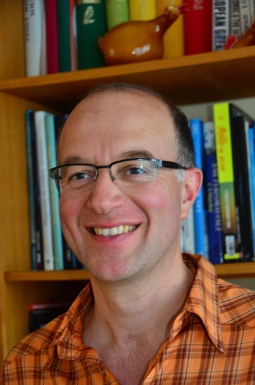
\includegraphics[scale=0.2]{npx.png} \hspace*{2.6cm} 
\includegraphics[scale=0.45]{esi.png}
\end{frame}

\begin{frame}
\frametitle{Table of contents}
\tableofcontents
\end{frame}

\section{DICOM viewers nowadays}

\begin{frame}
\frametitle{DICOM viewers nowadays}
It's very easy to find a DICOM viewer\\
But they all have one or more major issues :
\begin{itemize}
\item[•] Not free software;
\item[•] Expensive;
\item[•] Not user-friendly or unadapted GUI;
\item[•] Platform restriction;
\item[•] Lack of approval for medical diagnosis;
\item[•] Negligence towards the user.
\item[•] Only reads some DICOM files
\end{itemize}
\end{frame}

\section{What do we want?}

\begin{frame}
\frametitle{What do we want?}
\begin{itemize}
\item[•] Approval for medical diagnosis (CE Marked / FDA Approved)
\item[•] Comfortable and intuitive
\item[•] Focus is put towards the user experience
\item[•] Free software, all features included
\item[•] Cross-platform
\item[•] Customizable and have presets for each specialty
\item[•] Able to read each dicom file (even proprietary fields)
\item[•] AGPL (Affero General Public License)
\end{itemize}
\end{frame}

\section{Inspiration}

\subsection{Osirix}

\begin{frame}
\frametitle{Osirix}

\includegraphics[scale=0.17]{Osirix.jpg}
\begin{itemize}
\item[•] Developped by a doctor, Antoine Rosset
\item[•] Appreciated by the professionals
\item[•] Restricted to Mac OS X
\end{itemize}
\end{frame}

\subsection{Other viewers}

\begin{frame}
\frametitle{Other viewers}
\begin{tabular}{>{\centering\arraybackslash}m{.2\textwidth} >{\centering\arraybackslash}m{.2\textwidth} >{\centering\arraybackslash}m{.2\textwidth} >{\centering\arraybackslash}m{.2\textwidth}}
3D Slicer & 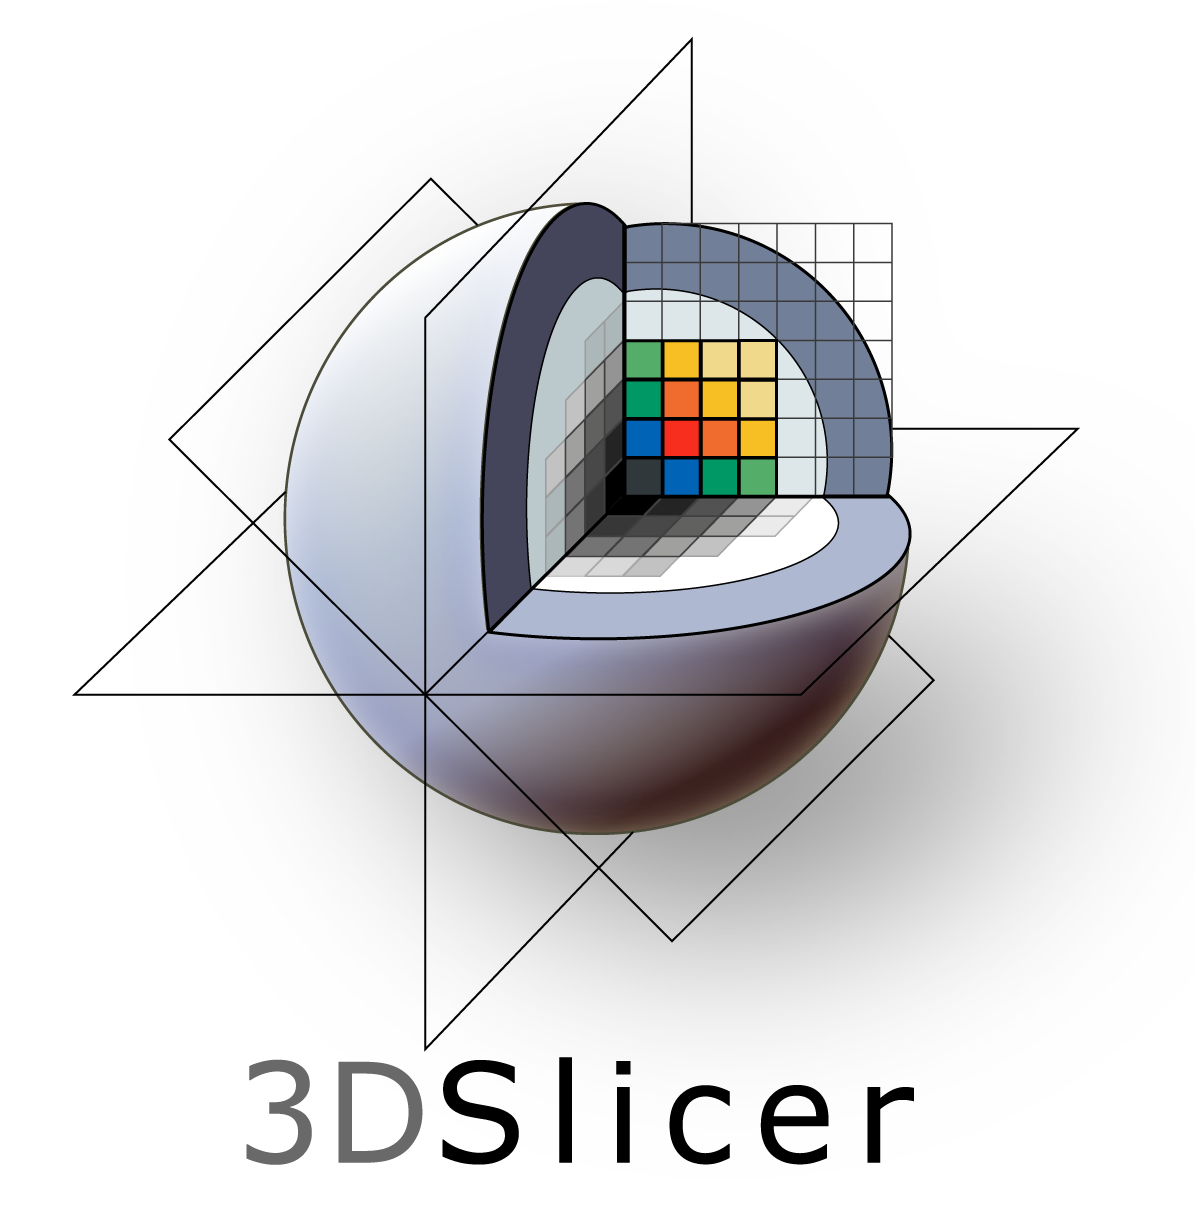
\includegraphics[width=2.6cm]{slicer.png} & Ginkgo CADx & 
\includegraphics[width=1.7cm]{ginkgo.png}\\
VR-Render & 
\includegraphics[width=2.2cm]{vrrender.png} & MedInria & 
\includegraphics[width=2.5cm]{medinria.png}
\end{tabular}
\end{frame}

\subsection{Orthanc}

\begin{frame}
\frametitle{Orthanc}

\includegraphics[scale=0.15]{Orthanc.png}
\begin{itemize}
\item[•] Belgian project
\item[•] Created by Sébastien Jodogne
\item[•] 2014 Free Software Award winner
\item[•] DICOM server for medical imaging
\item[•] GPL license
\item[•] OrthancViewer (Quentin Smetz)
\end{itemize}
\end{frame}

\section{Our tools}

\begin{frame}
\frametitle{Our tools}
\begin{itemize}
\item[•] C++
\item[•] Qt (LGPL)
\item[•] VTK (BSD)
\item[•] ITK (Apache 2.0)
\item[•] GDCM (BSD)
\end{itemize}
There are natural bridge classe(s) for Qt/VTK and GDCM/VTK/ITK
\end{frame}

\section{Features}

\begin{frame}
\frametitle{}Features
Non exhaustive list, can be altered during the development 
\begin{itemize}
\item[•] Image manipulations on each plane (axial, coronal, sagittal)
\item[•] 3D Volume Rendering (Raycasting, MIP, MPR)
\item[•] 3D Volume manipulation (Zoom, Rotation, ...)
\item[•] PET-CT Merge
\item[•] Hounsfield windowing
\item[•] Colormapping
\item[•] 2D+t / 3D+t files handling
\end{itemize}
\end{frame}

\section{Conclusion}

\begin{frame}
\frametitle{Conclusion}
MediVisu will be a universal DICOM image viewer and analyzer, certified, comfortable and cross-platform.
It will be a free software under AGPL.
\end{frame}

\begin{frame}
\frametitle{Contact us}
\begin{center}

\includegraphics[scale=0.7]{medivisu.png}
\end{center}
\begin{thebibliography}{10}
\beamertemplatearticlebibitems
\bibitem{MediVisu}
MediVisu
\newblock Contact us at {\tt medivisu-dev@pettiaux.be}
\end{thebibliography}
\end{frame}

\end{document}